\documentclass{article}
\usepackage{amsmath}
\usepackage{mathtools}
\usepackage{gensymb}
\usepackage[a4paper,inner=1.5cm,outer=1.5cm,top=2cm,bottom=0.5cm]{geometry} 
\usepackage{xcolor}
\usepackage{tikz}
\usepackage{multicol}
\usepackage{pgfplots}
\usetikzlibrary{intersections}
\usetikzlibrary{intersections,calc,angles,quotes}
\usetikzlibrary{calc,angles,positioning,intersections,quotes,decorations.markings}
\usepackage{tkz-euclide}
\usetikzlibrary{backgrounds}
\usetikzlibrary{calc,through}
\usetikzlibrary{angles}
\usetikzlibrary{fadings}
\usetikzlibrary{shapes.geometric}
\usetikzlibrary{shapes.symbols}
\usepackage{draftwatermark}
\usepackage{mathptmx}

\SetWatermarkText{\textcolor{black!10}{Mathema Shukur}}
\SetWatermarkFontSize{2 cm}
\usepackage[utf8]{inputenc}
\usepackage{fontspec}

\setmainfont{[Kalpurush.ttf]}
\newfontface{\en}{[Arial.ttf]} %%this is optional, if you want to use a secondary font. Any english font is supported
\newlength\Radius
\setlength\Radius{4cm}
\begin{document} 
	\Large
	\textcolor{red}{Welcome To} 
	\\
	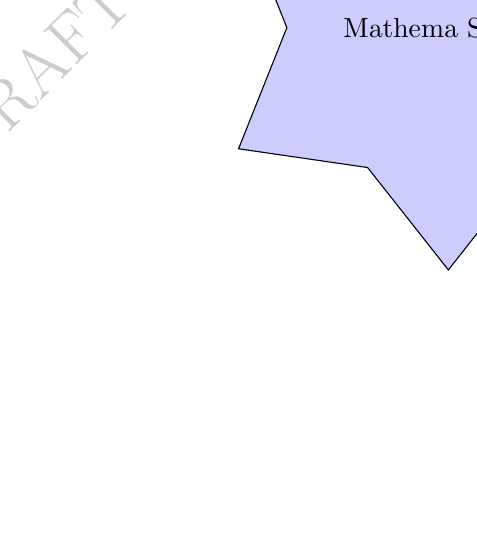
\begin{tikzpicture}
		\tikz \node [fill=blue!20,star,star points=6,draw] {Mathema Shukur };
	\end{tikzpicture}
	\\
  (১) $(-1,-1)$ বিন্দুটির পোলার স্থানাঙ্ক নির্ণয় কর।[বরিশাল বোর্ড-২০১৯]\\
  \begin{align*}
  & x=-1,\quad y=-1\\
  \\
 & r=\sqrt{x^2+y^2}\\
 & =\sqrt{(-1)^2+(-1)^2}\\
 & =\sqrt{1+1}\\
 & =\sqrt{2}\\ 
  \end{align*}
 
  বিন্দুটি ৩য় চতুর্ভাগে অবস্থিত\\
  \begin{align*}
  	\theta&=\pi+\tan^{-1}|\frac{y}{x}|\\
  	\theta&=\pi+\tan^{-1}|\frac{-1}{-1}|\\
  	\theta&=\pi+\tan^{-1} 1\\
  	\theta&=\pi+\frac{\pi}{4}\\
  	\theta&=\frac{5\pi}{4}\\
  \end{align*}
  সুতরাং, পোলার স্থানাঙ্ক,($\sqrt{2},\frac{5\pi}{4}$) \\ 
 (২)$y+x=0$ সরলরেখাটি  x অক্ষের ধনাত্মক দিকের সাথে কত ডিগ্রি কোণ উৎপন্ন করে।[বরিশাল বোর্ড-২০১৯]\\
  \begin{align*}
  	y+x&=0\\
  	y&=-x\\
  	&\boxed{\textcolor{blue}{y=mx+c}}\\
  	m&=-1\\
  	  	\tan \theta&=-1\\
  		\tan \theta&=\tan135\degree\\
  	\theta&=135\degree\\
  \end{align*}
(৩)$x+y=2$ এবং$y-x=0$ রেখাদ্বয়ের ছেদবিন্দুগামী এবং$x$ অক্ষের সমান্তরাল রেখার সমীকরণ নির্ণয় কর।[বরিশাল বোর্ড-২০১৯]\\
\begin{align*}
	y&=x\\
	x+y&=2\\
	x+x&=2\\
	2x&=2\\
	x&=1\\
	y&=1\\
\end{align*}
ছেদবিন্দুর স্থানাঙ্ক, $(1,1)$\\
$(1,1)$ বিন্দুগামী $x$ অক্ষের সমান্তরাল রেখার সমীকরণ,\\
$y=1$\\
$y-1=0$\\
(৪) $x-3y-8=0$ এবং $3x-y+7=0$ সরলরেখাদ্বয়ের  অন্তর্ভুক্ত সূক্ষ্মকোণের মান কত?[বরিশাল বোর্ড-২০১৯]\\
\begin{multicols}{2}
\begin{align*}
	x-3y-8&=0\\
	3y&=x-8\\
	y&=\frac{1}{3}x-\frac{8}{3}\\
	&\boxed{\textcolor{blue}{y=mx+c}}\\
	&m_1=\frac{1}{3}
\end{align*}
আবার,\\
\begin{align*}
	3x-y+7&=0\\
	y&=3x+7\\
	&\boxed{\textcolor{blue}{y=mx+c}}\\
	&m_2=3
\end{align*}
\end{multicols}
অন্তর্ভুক্ত কোণ $\theta$ হলে,\\
\begin{align*}
	\tan\theta&=\pm\frac{m_1-m_2}{1+m_1m_2}\\
	\tan\theta&=\pm\frac{\frac{1}{3}-3}{1+\frac{1}{3}.3}\\
	\tan\theta&=\pm\frac{\frac{-8}{3}}{2}\\
	\tan\theta&=\pm\frac{4}{3}\\
\end{align*}
সূক্ষ্মকোণ$,\theta$=$\tan^{-1}(\frac{4}{3}$)\\ 
\\ 
(বরিশাল বোর্ড-২০১৯)\\ 
(৫) $A(4,0)$ ও $B(0,3)$রেখাংশ $P$ ও $Q$ বিন্দুতে সমান তিন ভাগে অন্তর্বিভক্ত হয়।\\
(i)P বিন্দুর স্থানাংক নির্ণয় কর ?\\
(ii) OP এবং OQ সরলরেখাসমূহের সমীকরণ নির্ণয় কর । যেখানে o মূলবিন্দু \\ 
(iii) AB রেখার সমান্তরাল এবং $2\frac{2}{5}$একক দূরবর্তী সরলরেখার সমীকরণ নির্ণয় কর \\ 
\\
\begin{align*}
&	x_1=4,\quad y_1=0\\
&	x_2=0,\quad y_2=3\\
&m_1=1,\quad m_2=2
\end{align*}
$P$ বিন্দুর স্থানাঙ্ক, \\
\begin{align*}
	&\left(\frac{m_1\times x_2+m_2\times x_1}{m_1+m_2},\frac{m_1\times y_2+m_2\times y_1}{m_1+m_2}\right)\\
	&\left(\frac{1\times0+2\times4}{1+2},\frac{1\times3+2\times0}{1+2}\right)\\
&	\left(\frac{8}{3},\frac{3}{3}\right)\\
&	\left(\frac{8}{3},1\right)\\
\end{align*}
আবার,\\ 
$PB$এর মধ্যবিন্দু $Q$ এর স্থানাঙ্ক,\\
$\left(\frac{\frac{8}{3}+0}{2},\frac{1+3}{2}\right)$\\
$\left(\frac{4}{3},2\right)$\\
$OP$ রেখার সমীকরণ,\\
\begin{align*}
	\frac{x-0}{0-\frac{8}{3}}&=\frac{y-0}{0-1}\\
	3x&=8y\\
	3x-8y&=0\\
\end{align*}
$OQ$রেখার সমীকরণ, \\
\begin{align*}
	\frac{x-0}{0-\frac{4}{3}}&=\frac{y-0}{0-2}\\
	3x&=2y\\
	3x-2y&=0\\
\end{align*}
AB রেখার সমীকরণ,\\ 
$\frac{x}{4}+\frac{y}{3}=1$\\
$3x+4y-12=0$\\ 
সমান্তরাল রেখার সমীকরণ,\\
$3x+4y+K=0$
মধ্যবর্তী দূরত্ব,\\
\begin{align*}
	&\frac{|K-(-12)|}{\sqrt{3^2+4^2}}\\
	&=\frac{|K+12|}{5}\\
\end{align*}
প্রশ্নমতে,\\
\begin{align*}
	\frac{|K+12|}{5}&=2\frac{2}{5}\\
	\frac{K+12}{5}&=\pm\frac{12}{5}\\
     K+12&=\pm12\\
	K&=24,0\\
\end{align*}
$3x+4y-24=0$\\
$3x+4y=0$\\
\end{document}